\documentclass{article}
\usepackage[spanish]{babel}
\usepackage[a4paper,
            top=2cm,
            bottom=2cm,
            left=3cm,
            right=3cm,
            headheight=36pt,
            nomarginpar,
            includehead,
            includefoot,
            ]{geometry}
\usepackage{graphicx}
\usepackage{parskip}
\usepackage{fancyhdr}
\usepackage{xcolor}
\usepackage{enumitem}
\usepackage[many, minted, listings]{tcolorbox}


% Opciones para entornos de código fuente
\definecolor{bg}{RGB}{29, 35, 49}
\definecolor{framecolor}{RGB}{125, 138, 151}

\newtcbinputlisting{\inputcode}[3][]{
    listing only,
    listing engine=minted,
    listing file={#3},
    minted language={#2},
    minted style=lightbulb,
    breakable,
    colback=bg,
    colframe=framecolor,
    #1
}


% Opciones para entornos de pseudocódigo
\lstset{
    breakatwhitespace=true,             % sets if automatic breaks should only happen at whitespace
    breaklines=true,                    % sets automatic line breaking
    keepspaces=true,                    % keeps spaces in text, useful for keeping indentation of code (possibly needs columns=flexible)
    columns=flexible,
    escapechar=|,
    literate=   {á}{{\'a}}1             % corrige errores de utf-8
                {é}{{\'e}}1
                {í}{{\'i}}1
                {ó}{{\'o}}1
                {ú}{{\'u}}1,
}


% Encabezado y pie de página
\fancyhf{}
\lhead{
\includegraphics[height=32pt]{img/logo-uncuyo-fing.pdf}}
\rhead{ Licenciatura en Ciencias de la Computación \\
        Algoritmos y Estructuras de Datos II \\
        TP N\textsuperscript{o} 1: Análisis de Complejidad}
\rfoot{\thepage}
\pagestyle{fancy}


\begin{document}
{\centering
    {\bfseries\Large Universidad Nacional de Cuyo \par}
    \vspace{-0.2cm}
    {\bfseries\Large Facultad de Ingeniería \par}
    \vspace{-0.2cm}
    {\bfseries\Large Licenciatura en Ciencias de la Computación \par}
    \pagestyle{plain}
    \vfill
    \noindent\hrulefill \\
    {\scshape\Huge Trabajo Práctico N\textsuperscript{\Large\underline o} 1\par} % Título
    \vspace{0.5cm}
    {\scshape\Large Algoritmos y Estructuras de Datos \par}
    {\scshape\large Análisis de Complejidad \par}
    \vspace{0.5cm}
    {\scshape\Large 2024 \par} % Semestre
    \noindent\hrulefill \\
    \vspace{4cm}
    {\Large Gonzalo Padilla Lumelli \par}
    {\large Abril 2024 \par} % esto crea la fecha de hoy
    \vfill
    \setcounter{page}{1}
    \newpage
}


\subsection*{Ejercicio 1}
Demuestre que $6n^3 \neq O(n^2)$.

\subsubsection*{Solución}
$6n^3 = O(n^2)$ es, por definición, equivalente a decir que existen valores $c$ y $n_0$ tal que $6n^3 < c n^2$ para todo $n > n_0$. Se quiere demostrar lo opuesto, es decir, que para todo $c$ y $n_0$, existe $n > n_0$ tal que $6n^3 \geq c n^2$. Analizamos los puntos en los que $6n^3$ y $cn^2$ coinciden, y los intervalos definidos por tales puntos:

\begin{align*}
    6n^3 &= cn^2 \\
    6n^3 - cn^2 &= 0 \\
    n^2 \left (n - \frac{c}{6}\right ) &= 0
\end{align*}

Puede verse que ambas funciones son iguales en $n = 0$ y $n = c/6$. Para $n > c/6$, la diferencia es no negativa y, por lo tanto, $6n^3 \geq c n^2$. Si $n_0 \leq c/6$, entonces basta tomar $n = \lfloor c/6 \rfloor + 1 \geq n_0$, y se tendrá que $n > n_0$, y $6n^3 \geq c n^2$. Si, en cambio, $n_0 > c/6$, basta tomar $n = n_0 + 1 > c/6$, y se tendrá también que $n > n_0$, y $6n^3 \geq c n^2$.

Entonces, $\forall c \forall n_0 \exists n : [(n > n_0) \land (6n^3 \geq c n^2)]$. Por lo tanto, $6n^3 \neq O(n^2)$.


\subsection*{Ejercicio 2}
¿Cómo sería un array de números (mínimo 10 elementos) para el mejor caso de la estrategia de ordenación Quicksort(n)?

\subsubsection*{Solución}
El mejor caso ocurre cuando el pivote elegido en cada iteración es la mediana de los valores, y no se repiten valores. De esta forma, en cada iteración, siempre se ordenarán 2 particiones de con la mitad de elementos que la anterior. Utilizando el método maestro, se puede determinar que el orden de complejidad en este caso será de $\Theta (n \log n)$.

Cómo debería ser el array para que esto ocurra dependerá del criterio con el que se elija el pivote. Si siempre se elige el elemento de la mitad del array, entonces el mejor caso será cuando la lista ya esté ordenada, o esté ordenada en sentido inverso. Si se elige como pivote al primer o al último elemento, entonces el arreglo deberá tener en cada partición a su mediana como primer o último elemento, respectivamente, para cada posible partición binaria con la misma cantidad de elementos.


\subsection*{Ejercicio 3}
Cuál es el tiempo de ejecución de la estrategia Quicksort(A), Insertion-Sort(A) y Merge-Sort(A) cuando todos los elementos del array A tienen el mismo valor?

\subsubsection*{Solución}
En el caso de Quicksort, si todos los elementos tienen el mismo valor, se tendrá su peor caso, que es $O(n^2)$, ya que en cada iteración se colocará a todos los elementos a un lado del pivote, por lo que en la siguiente iteración deberán ordenarse $n-1$ elementos, dando un tiempo de ejecución de $T(n) = n + (n-1) + \dots + 2 + 1 = O(n^2)$

En el caso de Insertion-Sort, el tiempo de ejecución será $T(n) = O(n)$, ya que el mismo va ordenando elementos de a uno en uno, generando una porción del arreglo que ya está ordenada. Si el elemento que está analizando es mayor o igual que el último ya ordenado, lo salteará. Como todos los elementos son iguales, Insertion-Sort iterará sobre cada elemento una sola vez, sin cambiarlo de posición, y finalizará.

Merge-Sort {\em siempre} tiene un tiempo de ejecución del orden $\Theta (n \log n)$, independientemente de los elementos que contenga el array.


\subsection*{Ejercicio 4}
Implementar un algoritmo que ordene una lista de elementos donde siempre el elemento del medio de la lista contiene antes que él en la lista la mitad de los elementos menores que él. Explique la estrategia de ordenación utilizada.

\textbf{Ejemplo de lista de salida}

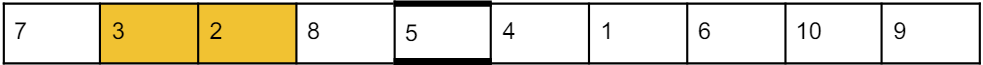
\includegraphics[width=400px]{./img/ejemploEjercicio4.png}

\subsubsection*{Solución}

\inputcode{python3}{./code/snippets/ejercicio4.py}


\subsection*{Ejercicio 5}
Implementar un algoritmo Contiene-Suma(A,n) que recibe una lista de enteros A y un entero n y devuelve True si existen en A un par de elementos que sumados den n. Analice el costo computacional.

\subsubsection*{Solución}

Primero ordenamos la lista, que es una operación de orden $O(n \log n)$. Luego la recorremos desde ambos extremos, verificando si la suma de el par de elementos actual es igual n. Si lo es, retornamos verdadero. Si es menor, avanzamos un paso desde la izquierda y verificamos nuevamente. Si es mayor, avanzamos desde la derecha. Si los punteros se encuentran, entonces no hay par de elementos que sumen $n$, entonces retornamos verdadero. La lista se recorre una sola vez, por lo que esta operación es de orden $O(n)$. Entonces, el orden de toda la operación está determinado por haber ordenado la lista, por lo tanto es de orden $O(n \log n)$.

\inputcode{python3}{./code/snippets/ejercicio5.py}


\subsection*{Ejercicio 6}
Investigar otro algoritmo de ordenamiento como BucketSort, HeapSort o RadixSort, brindando un ejemplo que explique su funcionamiento en un caso promedio. Mencionar su orden y explicar sus casos promedio, mejor y peor.

\subsubsection*{Solución}


\subsection*{Ejercicio 7}
A partir de las siguientes ecuaciones de recurrencia, encontrar la complejidad expresada en $\Theta (n)$ y ordenarlas de forma ascendente respecto a la velocidad de crecimiento. Asumiendo que $T(n)$ es constante para $n \leq 2$. Resolver 3 de ellas con el método maestro completo: $T(n) = a T(n/b) + f(n)$ y otros 3 con el método maestro simplificado: $T(n) = a T(n/b) + n^c$

\subsubsection*{Solución}
\begin{enumerate}[label=\alph*.]
    \item $T(n) = 2T(n/2) + n^4$
    
    Utilizando el método maestro simplificado tenemos que, $a=2$, $b=2$, $c=4$ y $\log_b a = \log_2 2 = 1 < c$, entonces se concluye que $T(n) = \Theta (n^c) = \Theta (n^4)$.


    \item $T(n) = 2T(7n/10) + n$
    
    Utilizando el método maestro simplificado tenemos que, $a=2$, $b=10/7$, $c=1$ y $\log_b a = \log_{10/7} 2 > 1.94 > c$, entonces se concluye que $T(n) = \Theta (n^{\log_b a}) = \Theta (n^{\log_{10/7} 2}) \approx \Theta (n^{1.94})$.

    
    \item $T(n) = 16T(n/4) + n^2$
    
    Utilizando el método maestro simplificado tenemos que, $a=16$, $b=4$, $c=2$ y $\log_b a = \log_4 16 = 2 = c$, entonces se concluye que $T(n) = \Theta (n^c \log n) = \Theta (n^2 \log n)$.


    \item $T(n) = 7T(n/3) + n^2$
    
    Utilizando el método maestro completo tenemos que, $a=7$, $b=3$, $f(n)=n^2$, y $\log_b a = \log_3 7 \approx 1.77$. Puede verse que $f(n)=n^2$ es acotable inferiormente por $n^{\log_b a + \epsilon} \approx n^{1.77 + \epsilon}$, con $\epsilon = 0.1 > 0$, por lo tanto, $f(n) = \Omega (n^{\log_b a + \epsilon})$. Además, se cumple que $af(n/b) = 7f(n/3) = 7 n^2 / 9 \leq c n^2$ para $c = 1 \leq 1$ y todo $n$. Entonces, se cumple el tercer caso del método maestro, y se concluye que $T(n) = \Theta (f(n)) = \Theta (n^2)$.


    \item $T(n) = 7T(n/2) + n^2$
    
    Utilizando el método maestro completo tenemos que, $a=7$, $b=2$, $f(n)=n^2$, y $\log_b a = \log_2 7 \approx 2.81$. Puede verse que $f(n)=n^2$ es acotable superiormente por $n^{\log_b a - \epsilon} \approx n^{2.81 - \epsilon}$, con $\epsilon = 0.5 > 0$, por lo tanto, $f(n) = O(n^{\log_b a + \epsilon})$. Entonces, se cumple el primer caso del método maestro, y se concluye que $T(n) = \Theta (n^{\log_b a}) = \Theta (n^{\log_2 7}) \approx \Theta (n^{2.81})$.


    \item $T(n) = 2T(n/4) + \sqrt{n}$
    
    Utilizando el método maestro completo tenemos que, $a=2$, $b=4$, $f(n)=\sqrt{n}$, y $\log_b a = \log_4 2 = 0.5$. Puede verse que $f(n)=\sqrt{n}$ es acotable superior e inferiormente por $n^{\log_b a \pm \epsilon} = n^{0.5 \pm \epsilon}$ con $\epsilon = 0.1 > 0$, por lo tanto, $f(n) = \Theta (n^{\log_b a})$. Entonces, se cumple el segundo caso del método maestro, y se concluye que $T(n) = \Theta(n^{\log_b a} \log n) = \Theta (\sqrt{n} \log n)$.

\end{enumerate}

Finalmente, las ecuaciones quedan ordenadas de forma ascendente según su orden de complejidad de la siguiente manera:

\begin{enumerate}
    \item f. $T(n) = \Theta (\sqrt{n} \log n)$
    \item b. $T(n) = \Theta (n^{\log_{10/7} 2}) \approx \Theta (n^{1.94})$
    \item d. $T(n) = \Theta (n^2)$
    \item c. $T(n) = \Theta (n^2 \log n)$
    \item e. $T(n) = \Theta (n^{\log_2 7}) \approx \Theta (n^{2.81})$
    \item a. $T(n) = \Theta (n^4)$
\end{enumerate}


\end{document}
